\section*{Moving between types of solutions}
one can note that it is fairly straightforward to find certain types of solutions such as numerical solutions via Newton-Raphson, but sometimes it is more desirable to have symbolic solutions or parametric expressions of the variety. in the diagram below, we illustrate the different types of solutions and the methods we will use to move between them.

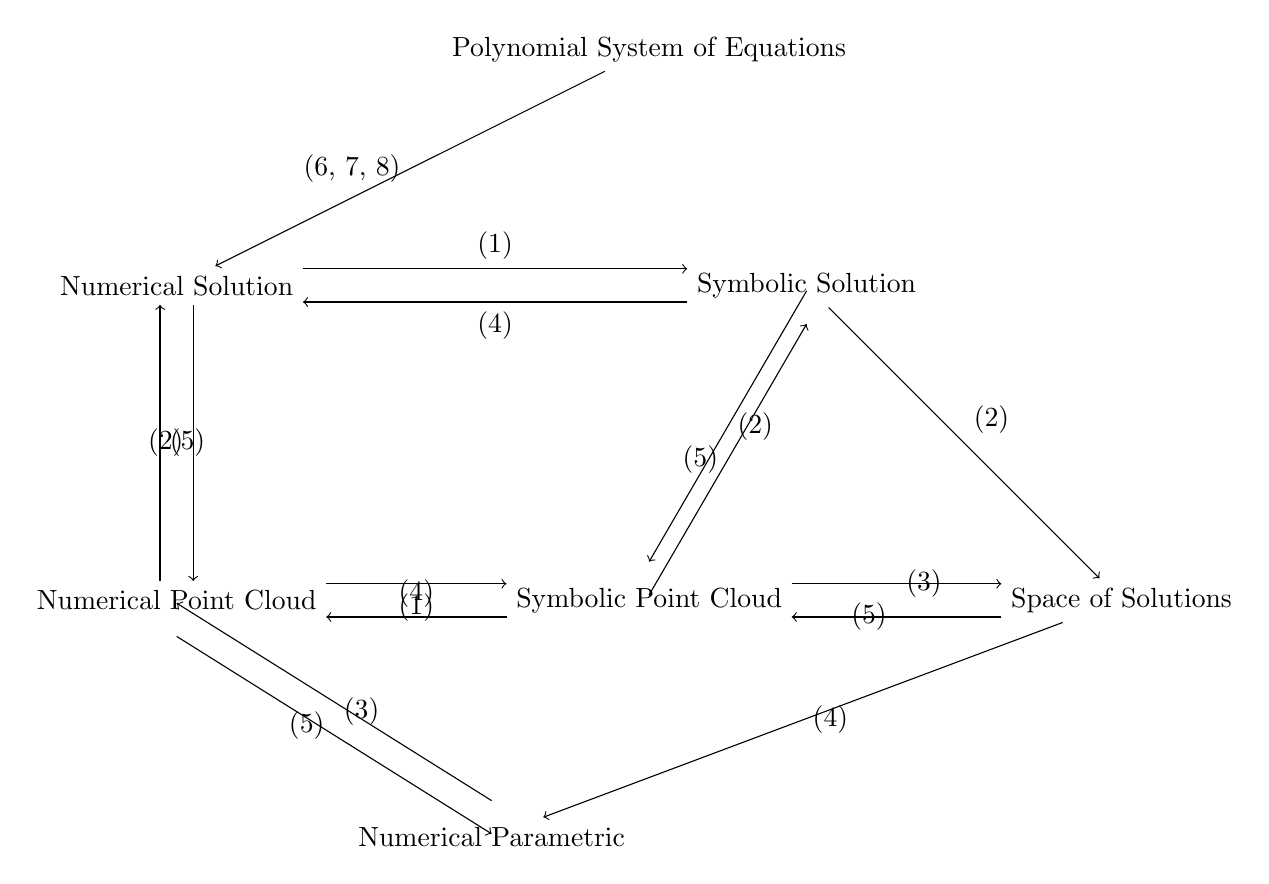
\begin{tikzpicture}[node distance=2cm]
  % spread out layout
  \node (start) at (6,0) {Polynomial System of Equations};
  \node (numerical) at (0,-3) {Numerical Solution};
  \node (symbolic) at (8,-3) {Symbolic Solution};
  \node (num_cloud) at (0,-7) {Numerical Point Cloud};
  \node (sym_cloud) at (6,-7) {Symbolic Point Cloud};
  \node (parametric) at (12,-7) {Space of Solutions};
  \node (num_parametric) at (4,-10) {Numerical Parametric};

  % Straight arrows (no bends)
  \draw[->] (start) -- (numerical) node[midway, left] {(6, 7, 8)};
  \draw[->] ([yshift=6pt]numerical.east) -- ([yshift=6pt]symbolic.west) node[midway, above] {(1)};
  \draw[->] ([yshift=-6pt]symbolic.west) -- ([yshift=-6pt]numerical.east) node[midway, below] {(4)};
  \draw[->] ([xshift=6pt]numerical.south) -- ([xshift=6pt]num_cloud.north) node[midway, left] {(2)};
  \draw[->] ([yshift=6pt]symbolic.south) -- ([yshift=6pt]sym_cloud.north) node[midway, right] {(2)};
  \draw[->] ([xshift=-6pt]num_cloud.north) -- ([xshift=-6pt]numerical.south) node[midway, right] {(5)};
  \draw[->] ([yshift=-6pt]sym_cloud.north) -- ([yshift=-6pt]symbolic.south) node[midway, left] {(5)};
  \draw[->] ([yshift=6pt]num_cloud.east) -- ([yshift=6pt]sym_cloud.west) node[midway, below] {(1)};
  \draw[->] ([yshift=-6pt]sym_cloud.west) -- ([yshift=-6pt]num_cloud.east) node[midway, above] {(4)};
  \draw[->] ([yshift=6pt]sym_cloud.east) -- ([yshift=6pt]parametric.west) node[midway, right] {(3)};
  \draw[->] ([yshift=-6pt]parametric.west) -- ([yshift=-6pt]sym_cloud.east) node[midway, left] {(5)};
  \draw[->] (symbolic) -- (parametric) node[midway, above right] {(2)};
  \draw[->] (parametric) -- (num_parametric) node[midway, right] {(4)};
  \draw[->] ([yshift=6pt]num_parametric.north) -- ([yshift=6pt]num_cloud.south) node[midway, below left] {(5)};
  \draw[->] ([yshift=-6pt]num_cloud.south) -- ([yshift=-6pt]num_parametric.north) node[midway, above right] {(3)};
\end{tikzpicture}


\begin{enumerate}
    \item \textbf{PSLQ and numerical fitting:} in this method, we use the PSLQ algorithm to find integer relations in the numerical solutions, replace numerical results with symbolic expressions, refit the solution and repeat until we have replaced all numerical values with symbolic expressions.
    \item \textbf{Going penpendicular to Jacobian null space:} given a solution to the polynomial system of equations, and if we will go in a direction that is perpendicular to the Jacobian null space at that point, we will remain in the solution space of the system. by taking small steps in such directions, we can sample more solutions to the system.
    \item \textbf{Symbolic regression:} given a point cloud of solutions, we can use symbolic regression to find parametric expressions that fit the point cloud.
    \item \textbf{Evaluating symbolic expressions:} given symbolic expressions, we can evaluate them to get numerical solutions.
    \item \textbf{Sampling points:} given numerical or symbolic parametric expressions of the variety, we can sample points from them to get point clouds of solutions.
    \item \textbf{SMT solvers:} SMT solvers can sometimes be used to find symbolic or numerical solutions to systems of equations.
    \item \textbf{Newton-Raphson:} given a system of equations, we can use the Newton-Raphson method to find numerical solutions to the system.
    \item \textbf{Homotopy continuation:} Homotopy continuation methods take a system of equations with known solutions and continuously deform it into the target system, tracking the solutions throughout the deformation process to find solutions to the original system.
\end{enumerate}
